% Options for packages loaded elsewhere
\PassOptionsToPackage{unicode}{hyperref}
\PassOptionsToPackage{hyphens}{url}
%
\documentclass[
]{article}
\usepackage{amsmath,amssymb}
\usepackage{lmodern}
\usepackage{iftex}
\ifPDFTeX
  \usepackage[T1]{fontenc}
  \usepackage[utf8]{inputenc}
  \usepackage{textcomp} % provide euro and other symbols
\else % if luatex or xetex
  \usepackage{unicode-math}
  \defaultfontfeatures{Scale=MatchLowercase}
  \defaultfontfeatures[\rmfamily]{Ligatures=TeX,Scale=1}
\fi
% Use upquote if available, for straight quotes in verbatim environments
\IfFileExists{upquote.sty}{\usepackage{upquote}}{}
\IfFileExists{microtype.sty}{% use microtype if available
  \usepackage[]{microtype}
  \UseMicrotypeSet[protrusion]{basicmath} % disable protrusion for tt fonts
}{}
\makeatletter
\@ifundefined{KOMAClassName}{% if non-KOMA class
  \IfFileExists{parskip.sty}{%
    \usepackage{parskip}
  }{% else
    \setlength{\parindent}{0pt}
    \setlength{\parskip}{6pt plus 2pt minus 1pt}}
}{% if KOMA class
  \KOMAoptions{parskip=half}}
\makeatother
\usepackage{xcolor}
\IfFileExists{xurl.sty}{\usepackage{xurl}}{} % add URL line breaks if available
\IfFileExists{bookmark.sty}{\usepackage{bookmark}}{\usepackage{hyperref}}
\hypersetup{
  pdftitle={Analysis of ZNF10 Spec-seq data},
  pdfauthor={Zheng Zuo},
  hidelinks,
  pdfcreator={LaTeX via pandoc}}
\urlstyle{same} % disable monospaced font for URLs
\usepackage[margin=1in]{geometry}
\usepackage{color}
\usepackage{fancyvrb}
\newcommand{\VerbBar}{|}
\newcommand{\VERB}{\Verb[commandchars=\\\{\}]}
\DefineVerbatimEnvironment{Highlighting}{Verbatim}{commandchars=\\\{\}}
% Add ',fontsize=\small' for more characters per line
\usepackage{framed}
\definecolor{shadecolor}{RGB}{248,248,248}
\newenvironment{Shaded}{\begin{snugshade}}{\end{snugshade}}
\newcommand{\AlertTok}[1]{\textcolor[rgb]{0.94,0.16,0.16}{#1}}
\newcommand{\AnnotationTok}[1]{\textcolor[rgb]{0.56,0.35,0.01}{\textbf{\textit{#1}}}}
\newcommand{\AttributeTok}[1]{\textcolor[rgb]{0.77,0.63,0.00}{#1}}
\newcommand{\BaseNTok}[1]{\textcolor[rgb]{0.00,0.00,0.81}{#1}}
\newcommand{\BuiltInTok}[1]{#1}
\newcommand{\CharTok}[1]{\textcolor[rgb]{0.31,0.60,0.02}{#1}}
\newcommand{\CommentTok}[1]{\textcolor[rgb]{0.56,0.35,0.01}{\textit{#1}}}
\newcommand{\CommentVarTok}[1]{\textcolor[rgb]{0.56,0.35,0.01}{\textbf{\textit{#1}}}}
\newcommand{\ConstantTok}[1]{\textcolor[rgb]{0.00,0.00,0.00}{#1}}
\newcommand{\ControlFlowTok}[1]{\textcolor[rgb]{0.13,0.29,0.53}{\textbf{#1}}}
\newcommand{\DataTypeTok}[1]{\textcolor[rgb]{0.13,0.29,0.53}{#1}}
\newcommand{\DecValTok}[1]{\textcolor[rgb]{0.00,0.00,0.81}{#1}}
\newcommand{\DocumentationTok}[1]{\textcolor[rgb]{0.56,0.35,0.01}{\textbf{\textit{#1}}}}
\newcommand{\ErrorTok}[1]{\textcolor[rgb]{0.64,0.00,0.00}{\textbf{#1}}}
\newcommand{\ExtensionTok}[1]{#1}
\newcommand{\FloatTok}[1]{\textcolor[rgb]{0.00,0.00,0.81}{#1}}
\newcommand{\FunctionTok}[1]{\textcolor[rgb]{0.00,0.00,0.00}{#1}}
\newcommand{\ImportTok}[1]{#1}
\newcommand{\InformationTok}[1]{\textcolor[rgb]{0.56,0.35,0.01}{\textbf{\textit{#1}}}}
\newcommand{\KeywordTok}[1]{\textcolor[rgb]{0.13,0.29,0.53}{\textbf{#1}}}
\newcommand{\NormalTok}[1]{#1}
\newcommand{\OperatorTok}[1]{\textcolor[rgb]{0.81,0.36,0.00}{\textbf{#1}}}
\newcommand{\OtherTok}[1]{\textcolor[rgb]{0.56,0.35,0.01}{#1}}
\newcommand{\PreprocessorTok}[1]{\textcolor[rgb]{0.56,0.35,0.01}{\textit{#1}}}
\newcommand{\RegionMarkerTok}[1]{#1}
\newcommand{\SpecialCharTok}[1]{\textcolor[rgb]{0.00,0.00,0.00}{#1}}
\newcommand{\SpecialStringTok}[1]{\textcolor[rgb]{0.31,0.60,0.02}{#1}}
\newcommand{\StringTok}[1]{\textcolor[rgb]{0.31,0.60,0.02}{#1}}
\newcommand{\VariableTok}[1]{\textcolor[rgb]{0.00,0.00,0.00}{#1}}
\newcommand{\VerbatimStringTok}[1]{\textcolor[rgb]{0.31,0.60,0.02}{#1}}
\newcommand{\WarningTok}[1]{\textcolor[rgb]{0.56,0.35,0.01}{\textbf{\textit{#1}}}}
\usepackage{graphicx}
\makeatletter
\def\maxwidth{\ifdim\Gin@nat@width>\linewidth\linewidth\else\Gin@nat@width\fi}
\def\maxheight{\ifdim\Gin@nat@height>\textheight\textheight\else\Gin@nat@height\fi}
\makeatother
% Scale images if necessary, so that they will not overflow the page
% margins by default, and it is still possible to overwrite the defaults
% using explicit options in \includegraphics[width, height, ...]{}
\setkeys{Gin}{width=\maxwidth,height=\maxheight,keepaspectratio}
% Set default figure placement to htbp
\makeatletter
\def\fps@figure{htbp}
\makeatother
\setlength{\emergencystretch}{3em} % prevent overfull lines
\providecommand{\tightlist}{%
  \setlength{\itemsep}{0pt}\setlength{\parskip}{0pt}}
\setcounter{secnumdepth}{-\maxdimen} % remove section numbering
\ifLuaTeX
  \usepackage{selnolig}  % disable illegal ligatures
\fi

\title{Analysis of ZNF10 Spec-seq data}
\author{Zheng Zuo}
\date{Aug 17, 2020}

\begin{document}
\maketitle

{
\setcounter{tocdepth}{2}
\tableofcontents
}
\hypertarget{background-and-experimental-design}{%
\subsection{Background and Experimental
design}\label{background-and-experimental-design}}

Human ZNF10 is a KRAB- zinc finger protein (ZFP) consisting of 10 C2H2
fingers. Based on ChIP-seq analysis by Abhi, B1H motif prediciton and
the cross-comparison between the two, it is likely that its finger one
to finger eight recognize the underlying motif in some irregular
configuration with some internal bases missing as shown below.

To verify this irregular recognition model, I made expression construct
to express the truncated F1-F8 of human ZNF10, and designed Spec-seq
libraries to randomize each position based on predicted ChIP-seq motifs
(UCD-1 to UCD-5). We can artificially designate portion of the predicted
motif as Upstream (ATATGGTG), Core (TGAG), and Downstream (GTAGGGGT)
respectively. Based on my previous work, it is very likely that ZNF10
also has the feature of dependent recognition, i.e., the proper
recognition of Upstream or Downstream motif depends on the presense of
intact core site (TGAT), so I included additional UCD-5N library to test
this hypothesis. Under this Upstream-Core-Downstream notation, the
regular B1H-predicted site can be designated as Upstream-1bp
spacer-Core-3bp spacer-Downstream (U1C3D), so I included five different
libraries to test the relative binding preference of ZNF10 for different
spacing formats including both ChIP- and B1H- prediced sites.

\begin{figure}
\centering
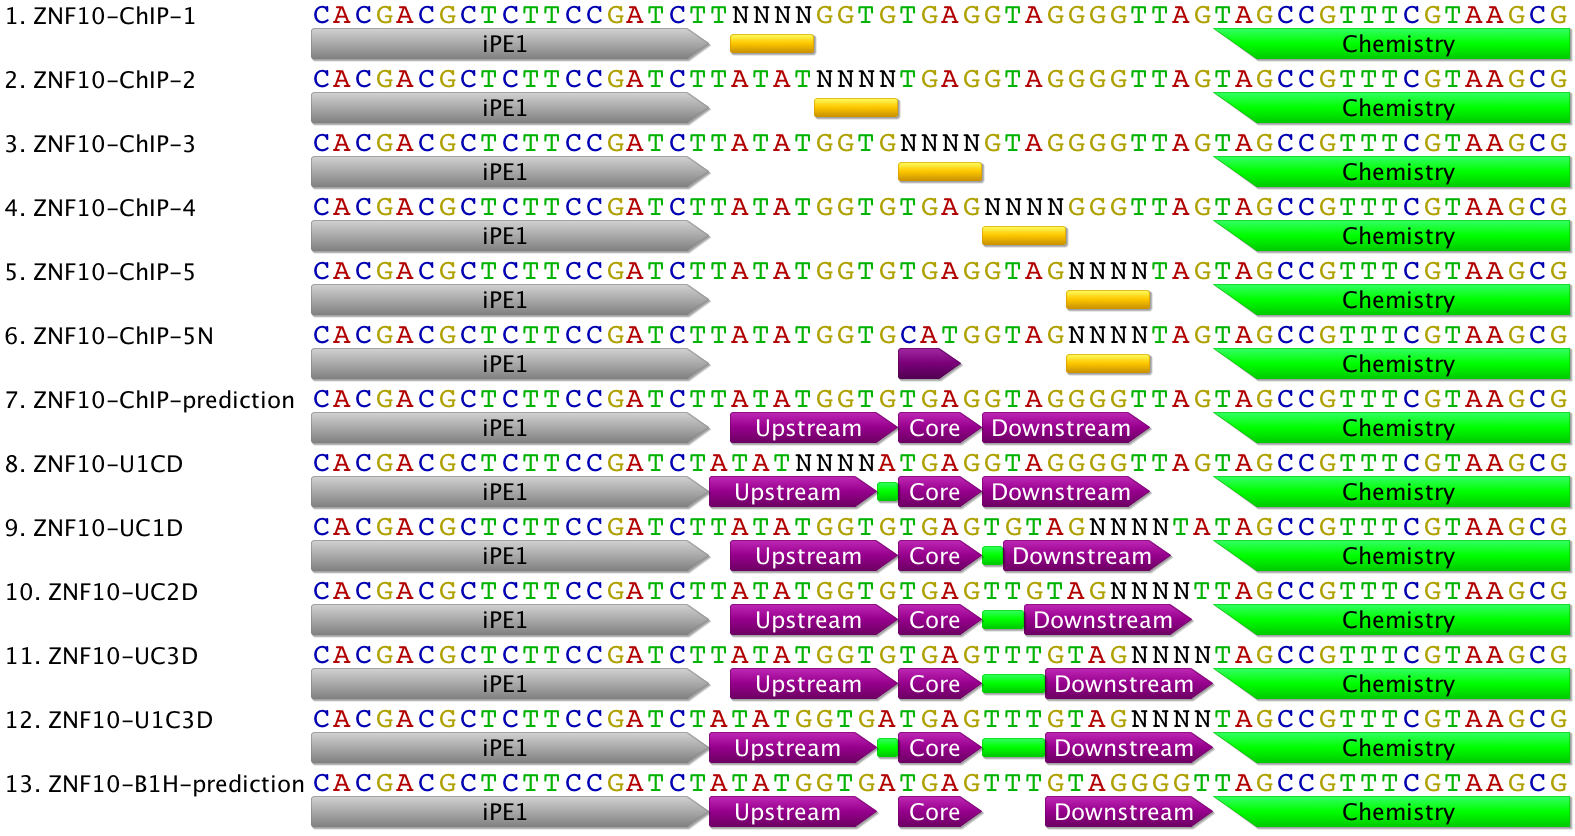
\includegraphics{ZNF10 libraries design.png}
\caption{Sequencing libraries design}
\end{figure}

\hypertarget{counting-sequences-from-raw-sequencing-files}{%
\subsection{Counting sequences from raw sequencing
files}\label{counting-sequences-from-raw-sequencing-files}}

\begin{Shaded}
\begin{Highlighting}[]
\FunctionTok{require}\NormalTok{(readr)}
\FunctionTok{require}\NormalTok{(dplyr)}

\NormalTok{Sample1.Bound }\OtherTok{\textless{}{-}} \FunctionTok{read\_csv}\NormalTok{(}\StringTok{"ZNF10.sample1.bound.raw"}\NormalTok{,}
  \AttributeTok{col\_names =} \ConstantTok{FALSE}
\NormalTok{) }\SpecialCharTok{\%\textgreater{}\%}
  \FunctionTok{count}\NormalTok{(}\AttributeTok{Sequence=}\FunctionTok{substring}\NormalTok{(X1, }\DecValTok{1}\NormalTok{, }\DecValTok{24}\NormalTok{), }\AttributeTok{name=}\StringTok{"Reads"}\NormalTok{)}

\NormalTok{Sample1.Unbound }\OtherTok{\textless{}{-}} \FunctionTok{read\_csv}\NormalTok{(}\StringTok{"ZNF10.sample1.unbound.raw"}\NormalTok{,}
  \AttributeTok{col\_names =} \ConstantTok{FALSE}
\NormalTok{) }\SpecialCharTok{\%\textgreater{}\%}
  \FunctionTok{count}\NormalTok{(}\AttributeTok{Sequence=}\FunctionTok{substring}\NormalTok{(X1, }\DecValTok{1}\NormalTok{, }\DecValTok{24}\NormalTok{), }\AttributeTok{name=}\StringTok{"Reads"}\NormalTok{)}

\NormalTok{Sample2.Bound }\OtherTok{\textless{}{-}} \FunctionTok{read\_csv}\NormalTok{(}\StringTok{"ZNF10.sample2.bound.raw"}\NormalTok{,}
  \AttributeTok{col\_names =} \ConstantTok{FALSE}
\NormalTok{) }\SpecialCharTok{\%\textgreater{}\%}
  \FunctionTok{count}\NormalTok{(}\AttributeTok{Sequence=}\FunctionTok{substring}\NormalTok{(X1, }\DecValTok{1}\NormalTok{, }\DecValTok{24}\NormalTok{), }\AttributeTok{name=}\StringTok{"Reads"}\NormalTok{)}

\NormalTok{Sample2.Unbound }\OtherTok{\textless{}{-}} \FunctionTok{read\_csv}\NormalTok{(}\StringTok{"ZNF10.sample2.unbound.raw"}\NormalTok{,}
  \AttributeTok{col\_names =} \ConstantTok{FALSE}
\NormalTok{) }\SpecialCharTok{\%\textgreater{}\%}
  \FunctionTok{count}\NormalTok{(}\AttributeTok{Sequence=}\FunctionTok{substring}\NormalTok{(X1, }\DecValTok{1}\NormalTok{, }\DecValTok{24}\NormalTok{), }\AttributeTok{name=}\StringTok{"Reads"}\NormalTok{)}
\end{Highlighting}
\end{Shaded}

\hypertarget{caculating-relative-binding-affinity-and-energy-based-on-bound-and-unbound-reads-for-each-variant.}{%
\subsubsection{Caculating relative binding affinity and energy based on
Bound and Unbound reads for each
variant.}\label{caculating-relative-binding-affinity-and-energy-based-on-bound-and-unbound-reads-for-each-variant.}}

\begin{Shaded}
\begin{Highlighting}[]
\NormalTok{Sample1.processed }\OtherTok{\textless{}{-}} 
  \FunctionTok{inner\_join}\NormalTok{(Sample1.Bound, Sample1.Unbound, }\AttributeTok{by =} \StringTok{"Sequence"}\NormalTok{) }\SpecialCharTok{\%\textgreater{}\%}
  \FunctionTok{mutate}\NormalTok{(}\AttributeTok{Library =}\NormalTok{ purrr}\SpecialCharTok{::}\FunctionTok{map\_chr}\NormalTok{(Sequence, library\_type)) }\SpecialCharTok{\%\textgreater{}\%}
  \FunctionTok{mutate}\NormalTok{(}\AttributeTok{Sequence =}\NormalTok{ purrr}\SpecialCharTok{::}\FunctionTok{map2\_chr}\NormalTok{(Sequence, Library, realign\_sequence)) }\SpecialCharTok{\%\textgreater{}\%}
\NormalTok{  dplyr}\SpecialCharTok{::}\FunctionTok{rename}\NormalTok{(}\AttributeTok{Bound =} \StringTok{\textquotesingle{}Reads.x\textquotesingle{}}\NormalTok{, }\AttributeTok{Unbound =} \StringTok{\textquotesingle{}Reads.y\textquotesingle{}}\NormalTok{) }\SpecialCharTok{\%\textgreater{}\%}
  \FunctionTok{filter}\NormalTok{(Bound}\SpecialCharTok{+}\NormalTok{Unbound }\SpecialCharTok{\textgreater{}=}\DecValTok{50}\NormalTok{, Library }\SpecialCharTok{!=} \StringTok{"Unclassified"}\NormalTok{) }\SpecialCharTok{\%\textgreater{}\%}
  \FunctionTok{mutate}\NormalTok{(}\StringTok{"B/Ub"} \OtherTok{=}\NormalTok{ Bound }\SpecialCharTok{/}\NormalTok{ Unbound,}
         \AttributeTok{pBound =}\NormalTok{ Bound}\SpecialCharTok{/}\FunctionTok{sum}\NormalTok{(Bound),}
         \AttributeTok{pUnbound =}\NormalTok{ Unbound}\SpecialCharTok{/}\FunctionTok{sum}\NormalTok{(Unbound),}
         \StringTok{"Relative Energy"} \OtherTok{=} \SpecialCharTok{{-}}\FunctionTok{log}\NormalTok{(Bound }\SpecialCharTok{/}\NormalTok{ Unbound),}
         \AttributeTok{Mismatch.ChIP =}\NormalTok{ TFCookbook}\SpecialCharTok{::}\FunctionTok{countMismatch}\NormalTok{(Sequence, ChIP.reference),}
          \AttributeTok{Mismatch.B1H =}\NormalTok{  TFCookbook}\SpecialCharTok{::}\FunctionTok{countMismatch}\NormalTok{(Sequence, B1H.reference)}
\NormalTok{         ) }\SpecialCharTok{\%\textgreater{}\%}
  \FunctionTok{arrange}\NormalTok{(}\StringTok{\textasciigrave{}}\AttributeTok{Relative Energy}\StringTok{\textasciigrave{}}\NormalTok{)}

\NormalTok{Sample1.processed}
\end{Highlighting}
\end{Shaded}

\begin{verbatim}
## # A tibble: 2,811 x 10
##    Sequence Bound Unbound Library `B/Ub`  pBound pUnbo~1 Relat~2 Misma~3 Misma~4
##    <chr>    <int>   <int> <chr>    <dbl>   <dbl>   <dbl>   <dbl>   <int>   <int>
##  1 ATATGGT~  5919     170 ChIP-4    34.8 1.15e-3 1.14e-4   -3.55       2       6
##  2 ATATTTT~  5488     191 ChIP-2    28.7 1.07e-3 1.28e-4   -3.36       3       7
##  3 ATATGGT~  5223     194 ChIP-4    26.9 1.02e-3 1.31e-4   -3.29       2       6
##  4 ATATGGT~  5403     226 ChIP-4    23.9 1.05e-3 1.52e-4   -3.17       1       5
##  5 ATATGGT~  2173      91 ChIP-4    23.9 4.24e-4 6.12e-5   -3.17       3       7
##  6 ATATGGT~  2762     120 ChIP-3    23.0 5.39e-4 8.07e-5   -3.14       1       5
##  7 ATATGGT~  2460     108 ChIP-4    22.8 4.80e-4 7.27e-5   -3.13       2       6
##  8 ATATGGT~  3642     161 ChIP-3    22.6 7.10e-4 1.08e-4   -3.12       1       5
##  9 ATATGTT~  5058     228 ChIP-2    22.2 9.87e-4 1.53e-4   -3.10       2       6
## 10 ATATGGT~  2787     129 ChIP-4    21.6 5.44e-4 8.68e-5   -3.07       2       6
## # ... with 2,801 more rows, and abbreviated variable names 1: pUnbound,
## #   2: `Relative Energy`, 3: Mismatch.ChIP, 4: Mismatch.B1H
\end{verbatim}

\begin{Shaded}
\begin{Highlighting}[]
\CommentTok{\#write.csv(Sample1.processed, file = "ZNF10.replicate1.csv", row.names=FALSE)}
\end{Highlighting}
\end{Shaded}

\hypertarget{summary-of-sequencing-reads-in-bound-and-unbound-fractions-respectively}{%
\subsubsection{Summary of Sequencing reads in Bound and Unbound
fractions,
respectively}\label{summary-of-sequencing-reads-in-bound-and-unbound-fractions-respectively}}

\begin{Shaded}
\begin{Highlighting}[]
\NormalTok{Sample1.processed }\SpecialCharTok{\%\textgreater{}\%}
  \FunctionTok{group\_by}\NormalTok{(Library) }\SpecialCharTok{\%\textgreater{}\%}
  \FunctionTok{summarize}\NormalTok{(}\StringTok{"Number of variants in library"}\OtherTok{=}\FunctionTok{n}\NormalTok{(),}
            \StringTok{"Total Bound reads"}\OtherTok{=}\FunctionTok{sum}\NormalTok{(Bound),}
            \StringTok{"Total Unbound reads"}\OtherTok{=}\FunctionTok{sum}\NormalTok{(Unbound),}
            \StringTok{"Bound/Unbound"} \OtherTok{=} \FunctionTok{sum}\NormalTok{(Bound)}\SpecialCharTok{/}\FunctionTok{sum}\NormalTok{(Unbound))}
\end{Highlighting}
\end{Shaded}

\begin{verbatim}
## # A tibble: 11 x 5
##    Library `Number of variants in library` `Total Bound reads` Total U~1 Bound~2
##    <chr>                             <int>               <int>     <int>   <dbl>
##  1 ChIP-1                              255             2783984    450209   6.18 
##  2 ChIP-2                              255              453446    103896   4.36 
##  3 ChIP-3                              255              109153    111335   0.980
##  4 ChIP-4                              255              457090    144262   3.17 
##  5 ChIP-5                              256              485189    126369   3.84 
##  6 ChIP-5N                             255               52408     76084   0.689
##  7 U1C3D                               256               79584     66139   1.20 
##  8 U1CD                                256              501461    137952   3.64 
##  9 UC1D                                256               76089    163999   0.464
## 10 UC2D                                256               64228     70379   0.913
## 11 UC3D                                256               64382     35891   1.79 
## # ... with abbreviated variable names 1: `Total Unbound reads`,
## #   2: `Bound/Unbound`
\end{verbatim}

\begin{Shaded}
\begin{Highlighting}[]
\NormalTok{PEM.ZNF10.ChIP }\OtherTok{\textless{}{-}}
  \FunctionTok{inner\_join}\NormalTok{(Sample1.Bound, Sample1.Unbound, }\AttributeTok{by =} \StringTok{"Sequence"}\NormalTok{) }\SpecialCharTok{\%\textgreater{}\%}
  \FunctionTok{mutate}\NormalTok{(}\AttributeTok{Library =}\NormalTok{ purrr}\SpecialCharTok{::}\FunctionTok{map\_chr}\NormalTok{(Sequence, library\_type)) }\SpecialCharTok{\%\textgreater{}\%}
\NormalTok{  dplyr}\SpecialCharTok{::}\FunctionTok{rename}\NormalTok{(}\AttributeTok{Bound =} \StringTok{\textquotesingle{}Reads.x\textquotesingle{}}\NormalTok{, }\AttributeTok{Unbound =} \StringTok{\textquotesingle{}Reads.y\textquotesingle{}}\NormalTok{) }\SpecialCharTok{\%\textgreater{}\%}
  \FunctionTok{filter}\NormalTok{(Bound}\SpecialCharTok{+}\NormalTok{Unbound }\SpecialCharTok{\textgreater{}=}\DecValTok{50}\NormalTok{, Library }\SpecialCharTok{!=} \StringTok{"Unclassified"}\NormalTok{) }\SpecialCharTok{\%\textgreater{}\%}
  \FunctionTok{mutate}\NormalTok{(}\StringTok{"B/Ub"} \OtherTok{=}\NormalTok{ Bound }\SpecialCharTok{/}\NormalTok{ Unbound,}
         \StringTok{"Energy"} \OtherTok{=} \SpecialCharTok{{-}}\FunctionTok{log}\NormalTok{(Bound }\SpecialCharTok{/}\NormalTok{ Unbound),}
         \AttributeTok{Mismatch.ChIP =}\NormalTok{ TFCookbook}\SpecialCharTok{::}\FunctionTok{countMismatch}\NormalTok{(Sequence, }\StringTok{"TATATGGTGTGAGGTAGGGGTTAG"}\NormalTok{),}
\NormalTok{         ) }\SpecialCharTok{\%\textgreater{}\%}
  \FunctionTok{arrange}\NormalTok{(}\StringTok{\textasciigrave{}}\AttributeTok{Energy}\StringTok{\textasciigrave{}}\NormalTok{) }\SpecialCharTok{\%\textgreater{}\%}
\NormalTok{  dplyr}\SpecialCharTok{::}\FunctionTok{filter}\NormalTok{(Mismatch.ChIP }\SpecialCharTok{\textless{}=} \DecValTok{2}\NormalTok{) }\SpecialCharTok{\%\textgreater{}\%}
\NormalTok{  TFCookbook}\SpecialCharTok{::}\FunctionTok{buildEnergyModel}\NormalTok{() }\SpecialCharTok{\%\textgreater{}\%}
\NormalTok{  TFCookbook}\SpecialCharTok{::}\FunctionTok{as.PEM}\NormalTok{()}
\end{Highlighting}
\end{Shaded}

\begin{verbatim}
## Warning: Expected 72 pieces. Additional pieces discarded in 331 rows [1, 2, 3,
## 4, 5, 6, 7, 8, 9, 10, 11, 12, 13, 14, 15, 16, 17, 18, 19, 20, ...].
\end{verbatim}

\begin{verbatim}
## Warning in if (method == "linear") model = lm(Energy ~ . - Energy, data =
## processed.data) else if (method %in% : 条件的长度大于一,因此只能用其第一元素
\end{verbatim}

\begin{Shaded}
\begin{Highlighting}[]
\NormalTok{ZNF10.motif }\OtherTok{=}\NormalTok{ PEM.ZNF10.ChIP[,}\DecValTok{2}\SpecialCharTok{:}\DecValTok{21}\NormalTok{]}

\NormalTok{TFCookbook}\SpecialCharTok{::}\FunctionTok{plotEnergyLogo}\NormalTok{(PEM.ZNF10.ChIP)}
\end{Highlighting}
\end{Shaded}

\begin{verbatim}
## Warning in if (col_scheme == "classic") col_scheme =
## ggseqlogo::make_col_scheme(chars = c("A", : 条件的长度大于一,因此只能用其第一元
## 素
\end{verbatim}

\begin{verbatim}
## Warning: The `<scale>` argument of `guides()` cannot be `FALSE`. Use "none" instead as
## of ggplot2 3.3.4.
## i The deprecated feature was likely used in the ggseqlogo package.
##   Please report the issue at <https://github.com/omarwagih/ggseqlogo/issues>.
\end{verbatim}

\includegraphics{ZNF10-Processor_files/figure-latex/unnamed-chunk-7-1.pdf}

\begin{Shaded}
\begin{Highlighting}[]
\CommentTok{\#save(list = "ZNF10.motif", file = "ZNF10.motif.RData")}
\end{Highlighting}
\end{Shaded}

\hypertarget{build-motif-models-based-on-all-double-variants-of-chip-reference-site}{%
\subsection{Build motif models based on all double variants of
ChIP-reference
site}\label{build-motif-models-based-on-all-double-variants-of-chip-reference-site}}

\begin{Shaded}
\begin{Highlighting}[]
\NormalTok{plot.sample1.ChIP }\OtherTok{\textless{}{-}}\NormalTok{ Sample1.processed }\SpecialCharTok{\%\textgreater{}\%}
\NormalTok{  dplyr}\SpecialCharTok{::}\FunctionTok{filter}\NormalTok{(Library }\SpecialCharTok{\%in\%} \FunctionTok{c}\NormalTok{(}\StringTok{"ChIP{-}1"}\NormalTok{, }\StringTok{"ChIP{-}2"}\NormalTok{, }\StringTok{"ChIP{-}3"}\NormalTok{, }\StringTok{"ChIP{-}4"}\NormalTok{, }\StringTok{"ChIP{-}5"}\NormalTok{)) }\SpecialCharTok{\%\textgreater{}\%}
\NormalTok{  dplyr}\SpecialCharTok{::}\FunctionTok{filter}\NormalTok{(Mismatch.ChIP}\SpecialCharTok{\textless{}=}\DecValTok{2}\NormalTok{) }\SpecialCharTok{\%\textgreater{}\%}
  \FunctionTok{rename}\NormalTok{(}\AttributeTok{Energy=}\StringTok{\textasciigrave{}}\AttributeTok{Relative Energy}\StringTok{\textasciigrave{}}\NormalTok{) }\SpecialCharTok{\%\textgreater{}\%}
\NormalTok{  TFCookbook}\SpecialCharTok{::}\FunctionTok{buildEnergyModel}\NormalTok{() }\SpecialCharTok{\%\textgreater{}\%}
\NormalTok{  TFCookbook}\SpecialCharTok{::}\FunctionTok{getEnergyMatrix}\NormalTok{() }\SpecialCharTok{\%\textgreater{}\%}
\NormalTok{  TFCookbook}\SpecialCharTok{::}\FunctionTok{plotEnergyLogo}\NormalTok{() }\SpecialCharTok{+}
  \FunctionTok{ggtitle}\NormalTok{(}\StringTok{"Motif of ZNF10}\SpecialCharTok{\textbackslash{}n}\StringTok{Sample \#1, ChIP{-}(1{-}5) variants"}\NormalTok{) }\SpecialCharTok{+}
  \FunctionTok{annotate}\NormalTok{(}\StringTok{\textquotesingle{}segment\textquotesingle{}}\NormalTok{, }\AttributeTok{x =}\NormalTok{ .}\DecValTok{5}\NormalTok{, }\AttributeTok{xend=}\FloatTok{8.5}\NormalTok{, }\AttributeTok{y=}\SpecialCharTok{{-}}\FloatTok{1.5}\NormalTok{, }\AttributeTok{yend=}\SpecialCharTok{{-}}\FloatTok{1.5}\NormalTok{, }\AttributeTok{size=}\DecValTok{2}\NormalTok{) }\SpecialCharTok{+} 
  \FunctionTok{annotate}\NormalTok{(}\StringTok{\textquotesingle{}text\textquotesingle{}}\NormalTok{, }\AttributeTok{x=}\DecValTok{5}\NormalTok{, }\AttributeTok{y=}\SpecialCharTok{{-}}\FloatTok{1.4}\NormalTok{, }\AttributeTok{label=}\StringTok{\textquotesingle{}Upstream Motif\textquotesingle{}}\NormalTok{, }\AttributeTok{color =} \StringTok{"blue"}\NormalTok{) }\SpecialCharTok{+} 
  \FunctionTok{annotate}\NormalTok{(}\StringTok{\textquotesingle{}segment\textquotesingle{}}\NormalTok{, }\AttributeTok{x =} \DecValTok{10}\NormalTok{, }\AttributeTok{xend=}\FloatTok{13.2}\NormalTok{, }\AttributeTok{y=}\SpecialCharTok{{-}}\FloatTok{1.5}\NormalTok{, }\AttributeTok{yend=}\SpecialCharTok{{-}}\FloatTok{1.5}\NormalTok{, }\AttributeTok{size=}\DecValTok{2}\NormalTok{) }\SpecialCharTok{+} 
  \FunctionTok{annotate}\NormalTok{(}\StringTok{\textquotesingle{}text\textquotesingle{}}\NormalTok{, }\AttributeTok{x=}\FloatTok{11.6}\NormalTok{, }\AttributeTok{y=}\SpecialCharTok{{-}}\FloatTok{1.4}\NormalTok{, }\AttributeTok{label=}\StringTok{\textquotesingle{}Core Motif\textquotesingle{}}\NormalTok{, }\AttributeTok{color =} \StringTok{"red"}\NormalTok{) }\SpecialCharTok{+} 
  \FunctionTok{annotate}\NormalTok{(}\StringTok{\textquotesingle{}segment\textquotesingle{}}\NormalTok{, }\AttributeTok{x =} \FloatTok{16.5}\NormalTok{, }\AttributeTok{xend=}\FloatTok{24.5}\NormalTok{, }\AttributeTok{y=}\SpecialCharTok{{-}}\FloatTok{1.5}\NormalTok{, }\AttributeTok{yend=}\SpecialCharTok{{-}}\FloatTok{1.5}\NormalTok{, }\AttributeTok{size=}\DecValTok{2}\NormalTok{) }\SpecialCharTok{+} 
  \FunctionTok{annotate}\NormalTok{(}\StringTok{\textquotesingle{}text\textquotesingle{}}\NormalTok{, }\AttributeTok{x=}\DecValTok{20}\NormalTok{, }\AttributeTok{y=}\SpecialCharTok{{-}}\FloatTok{1.4}\NormalTok{, }\AttributeTok{label=}\StringTok{\textquotesingle{}Downstream Motif\textquotesingle{}}\NormalTok{, }\AttributeTok{color =} \StringTok{"brown"}\NormalTok{) }\SpecialCharTok{+} 
  \FunctionTok{theme}\NormalTok{(}\AttributeTok{plot.title =} \FunctionTok{element\_text}\NormalTok{(}\AttributeTok{hjust =} \FloatTok{0.5}\NormalTok{))}


\NormalTok{plot.sample1.ChIP}
\end{Highlighting}
\end{Shaded}

\includegraphics{ZNF10-Processor_files/figure-latex/unnamed-chunk-9-1.pdf}

\begin{Shaded}
\begin{Highlighting}[]
\CommentTok{\#ggsave("ZNF10.Sample1.logo.png", plot=last\_plot())}
\end{Highlighting}
\end{Shaded}


\end{document}
